\section{Results}
\label{sec:results}

The analysis proceeds in two phases. Phase~1 characterizes broad
conversational patterns---tool overhead ratios, amplification factors,
and token accounting---across the full 857-session corpus using session
transcript analysis. Phase~2 performs detailed API-level waste
decomposition on a smaller proxy-captured sample (5~sessions,
99~API calls) where we have full request payloads. The corpus-scale
projection (Section~\ref{sec:corpus-projection}) then bridges the two
phases, applying measured conversion constants from Phase~2 to the
full corpus to estimate fleet-wide addressable waste.
The conversion constant used for projection (bytes-to-token ratio)
is estimated from a broader proxy sample of 139~API calls.

\subsection{Phase 1: Conversation-Level Waste}
\label{sec:phase1}

\paragraph{Tool overhead.}
Across the full corpus, 79.4\% of conversation bytes are tool
results. Assistant text accounts for 12.7\% and user text for
7.9\%. Two independent measurements converge on this ratio
(78.2\% and 79.4\%), suggesting it is a stable property of the
workload, not an artifact of sampling.

\paragraph{Tool type concentration.}
Tool usage is extremely concentrated (Figure~\ref{fig:tool-adoption}).
\texttt{Read} accounts for 75\% of all tool output bytes (9{,}393
calls, mean 7{,}935 bytes per result). \texttt{Bash} accounts for
13.3\% (10{,}090 calls). All other tools contribute less than 5\%
each. This concentration has a direct implication: file content
read by the \texttt{Read} tool is the dominant source of
context bloat.

\begin{figure}[ht]
\centering
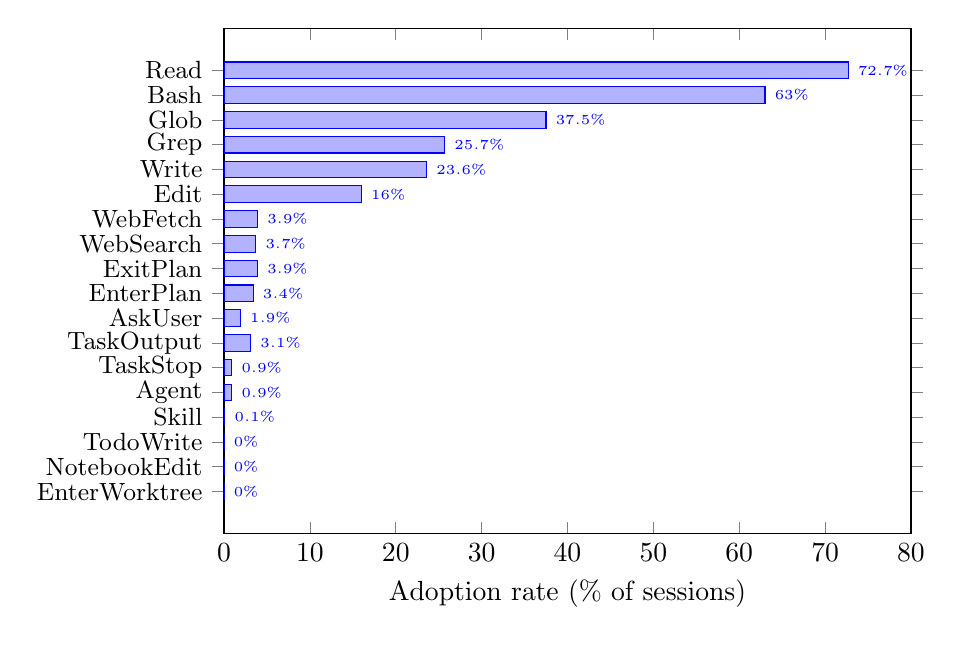
\begin{tikzpicture}
\begin{axis}[
    xbar,
    width=0.85\columnwidth,
    height=8cm,
    xlabel={Adoption rate (\% of sessions)},
    symbolic y coords={
        EnterWorktree, NotebookEdit, TodoWrite, Skill,
        Agent, TaskStop, TaskOutput, AskUser,
        EnterPlan, ExitPlan, WebSearch, WebFetch,
        Edit, Write, Grep, Glob, Bash, Read
    },
    ytick=data,
    yticklabel style={font=\small},
    xmin=0, xmax=80,
    bar width=6pt,
    nodes near coords={\pgfmathprintnumber\pgfplotspointmeta\%},
    nodes near coords style={font=\tiny, anchor=west},
    every axis plot/.append style={fill=blue!40},
]
\addplot coordinates {
    (0.0,EnterWorktree) (0.0,NotebookEdit) (0.0,TodoWrite)
    (0.1,Skill) (0.9,Agent) (0.9,TaskStop)
    (1.9,AskUser) (3.1,TaskOutput)
    (3.4,EnterPlan) (3.9,ExitPlan) (3.7,WebSearch)
    (3.9,WebFetch) (16.0,Edit) (23.6,Write)
    (25.7,Grep) (37.5,Glob) (63.0,Bash) (72.7,Read)
};
\end{axis}
\end{tikzpicture}
\caption{Tool adoption rate across 801 active sessions. The median
  session uses 3 of 18 available tools. Seven tools see zero or
  near-zero adoption, yet their full schemas (collectively
  $\sim$24{,}500 bytes) are sent on every API call.}
\label{fig:tool-adoption}
\end{figure}

\paragraph{Amplification factor.}
\label{sec:amplification}
Each tool result persists in context from the turn it was generated
until the session ends (or the client's internal compaction evicts
it). We define the \emph{amplification factor} as:
\[
  A = \frac{\sum_{r \in R} \text{size}(r) \times \text{turns\_survived}(r)}
           {\sum_{r \in R} \text{size}(r)}
\]
where $R$ is the set of tool results and turns\_survived is the
number of subsequent turns the result remains in context. This
measures how many times, on average, each byte of tool output is
reprocessed.

For main sessions: median $A = 84.4\times$, P75 $= 217.9\times$,
P90 $= 570.8\times$. For subagents: median $A = 12.8\times$
(short-lived, less accumulation). Amplification scales linearly
with session length at a ratio of approximately 0.5, confirming
the quadratic cost structure identified in recent
analyses~\citep{zeyliger2026quadratic}.

\paragraph{Token accounting.}
The corpus consumed 4.45~billion effective input tokens with a
93.5\% cache hit ratio, meaning the vast majority of input
processing is served from cache. However, cached tokens still
occupy the context window and require attention computation for
every output token. The average API call processes 82{,}061
effective input tokens and generates 88 output tokens---a
933:1 input-to-output ratio. Agentic coding is an overwhelmingly
input-bound workload.

\subsection{Phase 2: API-Level Waste Taxonomy}
\label{sec:taxonomy}

Using the proxy, we decompose 5 sessions (99 API calls, 24.4~MB
of request data) into four categories of addressable waste
(Table~\ref{tab:waste-taxonomy}).

\begin{table}[ht]
\centering
\caption{Waste taxonomy. Percentages are of total request bytes
  across 99 API calls.}
\label{tab:waste-taxonomy}
\small
\begin{tabular}{@{}lrrl@{}}
\toprule
\textbf{Category} & \textbf{Bytes} & \textbf{\%} & \textbf{Mechanism} \\
\midrule
Dead tool output & 6{,}468{,}360 & 26.5 & Stale results never re-referenced \\
Tool definition stubs & 4{,}924{,}950 & 20.2 & Schemas for unused tools \\
Static re-send & 2{,}680{,}794 & 11.0 & Unchanged system prompt content \\
Skill triplication & 700{,}582 & 2.9 & Same skill listed $3\times$ \\
\midrule
\textbf{Total addressable} & \textbf{14{,}774{,}686} & \textbf{60.5} & \\
\bottomrule
\end{tabular}
\end{table}

\paragraph{Dead tool output (26.5\%).}
Tool results from early turns persist in context long after any
reference to them. A file read during orientation (Q1 of the
session) survives approximately 90\% of the remaining session.
The content is reprocessed on every subsequent API call, consuming
attention without contributing to the current task.

\paragraph{Tool definition schemas (20.2\%).}
Claude Code sends 18 tool definitions totaling 63{,}088 bytes on
every API call. The median session uses 3 tools. The remaining 15
tool schemas ($\sim$52{,}500 bytes) are sent, tokenized, and
attended to on every call without ever being invoked.

\paragraph{Static system content (11.0\%).}
The system prompt, CLAUDE.md instructions, and memory files are
re-sent identically on every API call. While prompt caching avoids
the forward-pass cost, these tokens still occupy the context window
and participate in attention computation.

\paragraph{Skill triplication (2.9\%).}
The skills list---describing available slash commands---is injected
into messages three times under different prefixes (\texttt{base},
\texttt{example-skills:base}, \texttt{document-skills:base}).
Simple deduplication removes two-thirds of the entries.

\subsection{Interventions}
\label{sec:interventions}

All interventions operate in the proxy layer between the client
application and the inference API. No changes to the model, the
client, or the API are required.

\paragraph{Tool definition stubbing.}
Unused tool definitions are replaced with minimal stubs:
\begin{verbatim}
{"name": "NotebookEdit",
 "description": "...(first line)...",
 "input_schema": {"type":"object","properties":{}}}
\end{verbatim}
Full schemas ($\sim$3{,}505 bytes each) are replaced with stubs
($\sim$80 bytes). On first invocation of a stubbed tool, the full
definition is restored from a stored copy. The intervention is
session-scoped: once a tool is used, its schema remains restored
for the session. Per-request savings: $(18 - k) \times 3{,}425$
bytes, where $k$ is the number of tools used so far.

\paragraph{Content deduplication.}
Skill entries are parsed, grouped by base name, and deduplicated
(keeping the first occurrence). Saves 7{,}453 bytes per request.
Static system prompt components are tracked by content hash across
turns; identical components are logged as candidates for prefix
caching. Currently measurement-only for static components---actual
stripping requires cache-aware API support.

\paragraph{Stale result eviction (paging).}
Tool results older than a threshold (4 user-turns from the end of
the conversation) and larger than a minimum size (500 bytes) are
evicted. Error results are never evicted (the model needs them for
debugging). Evicted content is replaced with a summary:
\begin{quote}
\small
\texttt{[Paged out: Read /path/to/file.py (12{,}450 bytes, 287
  lines). Re-read if needed.]}
\end{quote}
The summary preserves the tool name, key parameter, and original
size ($\sim$200 bytes regardless of original size). If the model
re-invokes the same tool with the same parameters, this constitutes
a \emph{page fault}---the eviction was incorrect and the content
was still needed.

\subsection{Eviction Safety}
\label{sec:eviction}

We validate eviction safety through offline replay: 29
proxy-captured sessions are replayed through the pager, simulating
eviction decisions without making API calls.

\begin{table}[ht]
\centering
\caption{Eviction safety results from offline replay.}
\label{tab:eviction}
\small
\begin{tabular}{@{}lr@{}}
\toprule
Total simulated evictions & 1{,}393{,}000 \\
Page faults detected & 354 \\
\textbf{Fault rate} & \textbf{0.0254\%} \\
Content evicted & 8.49 GB \\
\bottomrule
\end{tabular}
\end{table}

A fault rate of 0.0254\% means the eviction policy is sound:
content older than 4 user-turns is almost never needed again. The
354 faults represent content that was genuinely dead by the age
criterion but happened to match a later request. A fault rate of
zero would indicate over-conservative eviction; some faults are
expected and acceptable.

\subsection{Live Treatment Comparison}
\label{sec:treatment}

We run a standardized task under three treatment conditions
(Table~\ref{tab:treatment}).

\begin{table}[ht]
\centering
\caption{Treatment comparison on a standardized task.}
\label{tab:treatment}
\small
\begin{tabular}{@{}lrrr@{}}
\toprule
\textbf{Metric} & \textbf{Baseline} & \textbf{Trimmed} & \textbf{Compact+Trim} \\
\midrule
API calls & 3 & 4 & 3 \\
Effective input tokens & 114{,}222 & 88{,}421 & 71{,}816 \\
Cache read tokens & 79{,}712 & 38{,}639 & 32{,}228 \\
Task completed correctly & Yes & Yes & Yes \\
\midrule
\textbf{Token reduction} & --- & 22.6\% & \textbf{37.1\%} \\
\bottomrule
\end{tabular}
\end{table}

The compact+trim treatment achieves 37.1\% reduction in effective
input tokens. Cache reads drop 59.6\%. The task completes correctly
under all conditions in this controlled run.

\subsection{Corpus-Scale Projection}
\label{sec:corpus-projection}

We validate the small-sample findings across the full 857-session
corpus using measured constants from the proxy sessions and tool
usage patterns extracted from raw session transcripts.

The bytes-to-token conversion ratio of 4.15 bytes per effective
input token is measured from 139 proxy-captured API calls.

\begin{table}[ht]
\centering
\caption{Corpus-scale token savings projection.}
\label{tab:corpus-tokens}
\small
\begin{tabular}{@{}lrr@{}}
\toprule
\textbf{Intervention} & \textbf{Tokens Saved} & \textbf{\% of Input} \\
\midrule
Tool stub trimming & 487.5M & 11.0\% \\
Skill deduplication & 95.8M & 2.2\% \\
Static re-send & 387.0M & 8.7\% \\
\midrule
\textbf{Total addressable} & \textbf{970.4M} & \textbf{21.8\%} \\
\bottomrule
\end{tabular}
\end{table}

The average saving is 17{,}913 tokens per API call. Across the
corpus, this translates to 85~billion fewer token-token attention
pairs (17{,}913 context tokens $\times$ 88 output tokens $\times$
54{,}170 calls).

\subsection{Production Deployment}
\label{sec:production}

We deploy \textsc{Pichay} in compact mode as the proxy for our own
development workflow---the system is used daily by the authors for
software engineering tasks. This section reports on two
representative sessions that illustrate different operating regimes.

\paragraph{Session A: Steady-state coding.}
A standard coding session using compact mode ($\tau = 4$,
$s_{\min} = 500$):

\begin{table}[ht]
\centering
\caption{Production Session A: steady-state coding.}
\label{tab:session-a}
\small
\begin{tabular}{@{}lr@{}}
\toprule
Context free before compaction & 7\% \\
Context free after compaction & 43\% \\
Total evictions & 15 \\
Garbage collected & 11 \\
Read evictions (pageable) & 4 \\
Page faults & 1 \\
Fault rate (Read only) & 25\% \\
\bottomrule
\end{tabular}
\end{table}

The session recovered 36~percentage points of context capacity---the
difference between imminent context exhaustion and substantial
remaining headroom. Of 15~evictions, 11~were garbage collection
(Bash/Grep/Glob outputs) and 4~were Read evictions. The single
fault was a plan file read early in the session and evicted when it
crossed the age threshold. The plan file is reference material
needed for the entire session---a hot page that FIFO treats as cold.
This is the classic working set failure: the eviction policy measures
age, not access pattern.

\paragraph{Session B: Sustained multi-agent coordination.}
A 681-turn session involving multiple subagent spawns and
cross-project file analysis:

\begin{table}[ht]
\centering
\caption{Production Session B: 681-turn sustained session.}
\label{tab:session-b}
\small
\begin{tabular}{@{}lr@{}}
\toprule
Turns & 681 \\
Evictions (total) & 680 \\
Garbage collected & 74 \\
Read evictions (pageable) & 606 \\
Page faults & 659 \\
\textbf{Fault rate (total evictions)} & \textbf{97\% (659/680)} \\
Peak compression & 5{,}038KB $\to$ 339KB \\
Session termination & API rate limit \\
\bottomrule
\end{tabular}
\end{table}

The 97\% fault rate is a pathology, not a feature. The system
evicted almost everything and the model re-requested almost
everything. Three specific patterns emerged:

\emph{Thrashing cycle.} Three files (3{,}438 + 1{,}570 + 1{,}592
bytes) were evicted and faulted in a cycle across turns 163--170+.
The working set exceeded the resident set---classic
thrashing~\citep{denning1968working}.

\emph{Sequential scan.} During a planning phase, the model read
across three code repositories, cycling through the same 7~files
repeatedly. The working set for planning was larger than what the
age threshold allowed to remain resident.

\emph{Self-inflicted inflation.} The 5{,}038KB pre-compaction size
includes re-reads caused by previous evictions. Without the
eviction-fault cycle, the original content would have been
substantially smaller. The proxy was measuring its own overhead as
``bytes saved''---a metric artifact of thrashing.

\emph{Cost.} The session terminated by hitting the API rate limit,
not the context limit. At 659~faults (each an inference-priced tool
call round-trip), thrashing consumed rate budget faster than useful
work. This demonstrates that fault cost is not merely computational
but monetary.

\paragraph{Anchor handle behavior.}
When a fresh model instance resumed a session containing paged-out
content, it stated: ``Let me re-read the files I need since some
were paged out, then create the task list and start implementing.''
The model recognized the retrieval handles, understood what was
missing, and chose to fault content in before acting---without any
instruction to do so. The handle format is self-describing: the
model infers the recovery mechanism from the text of the summary
alone.

% ====================================================================

\subsection{Cognitive Transaction Protocol Evaluation}
\label{sec:cognitive-transactions}

In a separate experiment track, we evaluate whether a model can operate
as a bounded cognitive transaction engine under an explicit
validator/reducer contract. The paper-ready tables are generated from
versioned artifacts under
\texttt{experiments/cognitive\_transactions/synthesis/}.

\paragraph{Phase 2: Candidate viability under protocol induction.}
Table~\ref{tab:ct-phase2} reports per-model validity with and without
synthetic teacher-trace guidance.

\begin{table}[ht]
\centering
\caption{Cognitive transactions Phase 2 (3 replicates, 15 steps per condition).}
\label{tab:ct-phase2}
\small
\begin{tabular}{@{}lrr@{}}
\toprule
\textbf{Model} & \textbf{Valid \% (none)} & \textbf{Valid \% (synthetic)} \\
\midrule
inception/mercury-2 & 6.7 & 100.0 \\
meta-llama/llama-4-maverick & 0.0 & 100.0 \\
allenai/olmo-3.1-32b-instruct & 0.0 & 100.0 \\
moonshotai/kimi-k2.5 & 0.0 & 73.3 \\
\bottomrule
\end{tabular}
\end{table}

The main result is an induction gap: under synthetic guidance, three of
four candidates reach 100\% valid transitions; without guidance, three of
four collapse to 0\% validity.

\paragraph{Phase 3: Guidance ablation and contract tightening.}
Table~\ref{tab:ct-phase3} shows that reduced guidance causes an abrupt
drop for OLMo-3 (86.7\% $\rightarrow$ 6.7\%), while focused contract
tightening recovers legality to 100\% in a larger retest.

\begin{table}[ht]
\centering
\caption{Cognitive transactions Phase 3 (OLMo-3).}
\label{tab:ct-phase3}
\small
\begin{tabular}{@{}lrrrr@{}}
\toprule
\textbf{Condition} & \textbf{Steps} & \textbf{Valid} & \textbf{Valid \%} & \textbf{Req-op misses} \\
\midrule
synthetic & 15 & 13 & 86.7 & 0 \\
synthetic\_reduced & 15 & 1 & 6.7 & 6 \\
synthetic\_followup & 25 & 23 & 92.0 & 0 \\
synthetic\_followup\_tweak & 50 & 50 & 100.0 & 0 \\
\bottomrule
\end{tabular}
\end{table}

\paragraph{Phase 4a: Realism and completion-budget interaction.}
Table~\ref{tab:ct-phase4} reports the corrected realism run
(\texttt{phase4\_20260311T173018Z}). No truncation or content-filter
events occurred in this run. The 2000 vs.~4000 setting is the per-step
completion token cap (\texttt{max\_tokens}), not the model context
window. Under this setting, task-dependent variations emerge:
4000 improves failure recovery, while 2000 performs better on long-horizon
durability and multitask contradiction reconciliation.

\begin{table}[ht]
\centering
\caption{Cognitive transactions Phase 4: working-set realism under induced handle recall (3 replicates per task/profile).}
\label{tab:ct-phase4}
\small
\begin{tabular}{@{}lrrr@{}}
\toprule
\textbf{Task} & \textbf{Valid \% @2000} & \textbf{Valid \% @4000} & \textbf{Delta (2000-4000)} \\
\midrule
failure\_recovery & 80.0 & 100.0 & -20.0 \\
long\_horizon\_durability & 86.7 & 83.3 & +3.3 \\
multitask\_benchmark & 72.2 & 66.7 & +5.6 \\
\bottomrule
\end{tabular}
\end{table}

This section supports a bounded claim: capability is real under protocol
scaffolding, but multitask contradiction handling remains the current
boundary and should be reported as a limitation.

A confirmatory rerun on 2026-03-11 (\texttt{phase4\_20260311T181454Z})
demonstrates run-to-run variance in cognitive transaction success while
preserving the same qualitative boundary. Relative to the corrected baseline
(\texttt{phase4\_20260311T173018Z}),
validity shifted by $-20.0$~points for failure\_recovery@4000
(100.0\%\,$\rightarrow$\,80.0\%) and $+5.6$~points for multitask\_benchmark@4000
(66.7\%\,$\rightarrow$\,72.2\%), with truncation/content-filter totals
remaining zero across all task/profile pairs.

\paragraph{Phase 4b: Working-set realism via handle recall.}
Separately, we implement a working-set realism mode where evicted handles
have explicit payload identity (hash, size) and \texttt{memory\_fault}
restores the full payload into the next-step input state. This enables
controlled working-set sweeps by varying evicted handle payload size
(\texttt{handle\_bytes}) while keeping completion caps high to avoid
structured-output truncation. A representative run with
\texttt{handle\_bytes}=5000 (\texttt{phase4\_20260311T194940Z}) reports
non-trivial recall volume alongside task success, making working-set usage
auditable in tokens and bytes.
